\documentclass[border=10pt]{standalone}
\usepackage{tikz}
\usetikzlibrary{arrows.meta, positioning, shapes.geometric, fit, backgrounds, calc}

% Dark-mode palette (light elements on transparent background)
\definecolor{srcblue}{HTML}{60A5FA}
\definecolor{docgold}{HTML}{FBBF24}
\definecolor{procgreen}{HTML}{34D399}
\definecolor{arrclr}{HTML}{94A3B8}
\definecolor{txtclr}{HTML}{E2E8F0}
\definecolor{dimtxt}{HTML}{9CA3AF}

\tikzset{
  state/.style={
    rectangle, rounded corners=6pt, draw=srcblue, line width=1.2pt,
    text=txtclr, font=\sffamily\bfseries,
    minimum width=26mm, minimum height=14mm, align=center
  },
  active/.style={
    rectangle, rounded corners=6pt, draw=procgreen, line width=1.2pt,
    text=txtclr, font=\sffamily\bfseries,
    minimum width=26mm, minimum height=14mm, align=center
  },
  optional/.style={
    rectangle, rounded corners=6pt, draw=docgold, line width=1.2pt,
    dashed,
    text=txtclr, font=\sffamily\bfseries,
    minimum width=26mm, minimum height=14mm, align=center
  },
  arr/.style={-{Stealth[length=5pt]}, thick, arrclr},
  lbl/.style={font=\sffamily\scriptsize, text=dimtxt},
}

\begin{document}
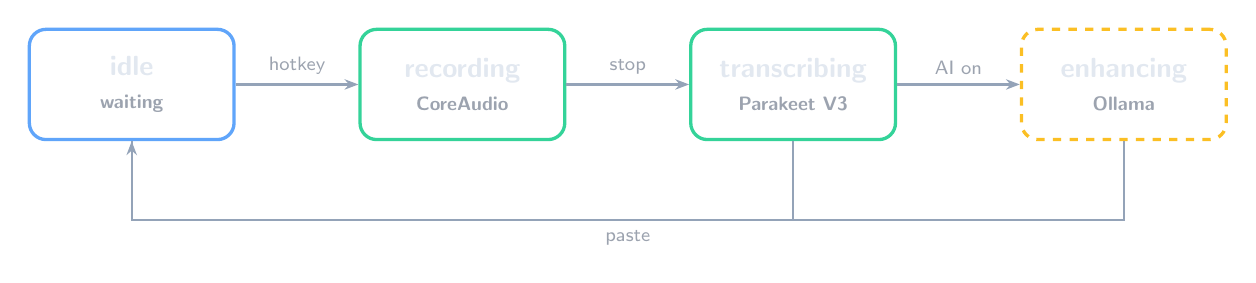
\begin{tikzpicture}

% --- States ---
\node[state] (idle) at (0,0) {idle\\{\scriptsize\color{dimtxt}waiting}};
\node[active] (recording) at (4.2,0) {recording\\{\scriptsize\color{dimtxt}CoreAudio}};
\node[active] (transcribing) at (8.4,0) {transcribing\\{\scriptsize\color{dimtxt}Parakeet V3}};
\node[optional] (enhancing) at (12.6,0) {enhancing\\{\scriptsize\color{dimtxt}Ollama}};

% --- Forward arrows ---
\draw[arr] (idle) -- node[lbl, above] {hotkey} (recording);
\draw[arr] (recording) -- node[lbl, above] {stop} (transcribing);
\draw[arr] (transcribing) -- node[lbl, above] {AI on} (enhancing);

% --- Return arrows ---
\draw[arrclr, thick] (transcribing.south) -- ++(0,-1) -| (idle.south);
\draw[arr] (enhancing.south) -- ++(0,-1) -| node[lbl, below, pos=0.25] {paste} (idle.south);

\end{tikzpicture}
\end{document}
